\chapter{同步和异步通信机制}\label{ch:sync-async-communication}

\section{同步和异步通信概述}\label{sec:5-sync-async-overview}

\subsection{同步通信概述}\label{subsec:5-sync-communication-overview}

操作系统中的同步（Synchronous）通信机制是用来同步两个并行或并发进程的一种机制。在传统操作系统中它通常表现为管道、信号量等机制。同步通信机制的最大特点为其阻塞性，也即一方发送后，另一方不接收，发送方即阻塞，直到接收方接收之后，发送方的阻塞才解除。如果接收方先接收，那么它也阻塞，直到发送方发送之后，接收方的阻塞才解除。采用这种传统实现的同步通信需要两个线程才能在进程之间通信。

在 RME 中，同步通信模型被进一步简化为线程迁移（Thread
Migration）调用\footnote{或说是本地过程调用}，其允许一个线程能够进入另一个进程内部执行一段代码后，再返回属于自己的进程继续执行。这是最高效的进程间通信（Inter-Process
Communication，IPC）实现之一。由于这种调用允许一个执行流跨越进程边界，因此只能在两个进程相当相互信任的情况下才能使用。其表观结果好像是一个进程内部运行的线程直接调用了另一个进程内部的函数，这样就只需要一个线程，也能够进行进程间通信。如果这个迁移调用要用到多余的参数，那么这些参数由共享内存、寄存器组或协处理器寄存器组传递。同步迁移调用是可以嵌套的，而且嵌套的层数可以是无限的。一个线程迁移的例子如下所示。该线程进行了两次迁移，并且在三个进程之间交替执行。图中的红色正三角代表迁移调用激活，红色倒三角代表迁移调用返回。在进程2和进程3中，线程执行流上的方框标注着线程的迁移调用栈，黑色三角指向的则是迁移调用栈的栈顶。在返回时，总是先返回到栈顶所指的进程内。

\begin{figure}[htbp]
    \centering
    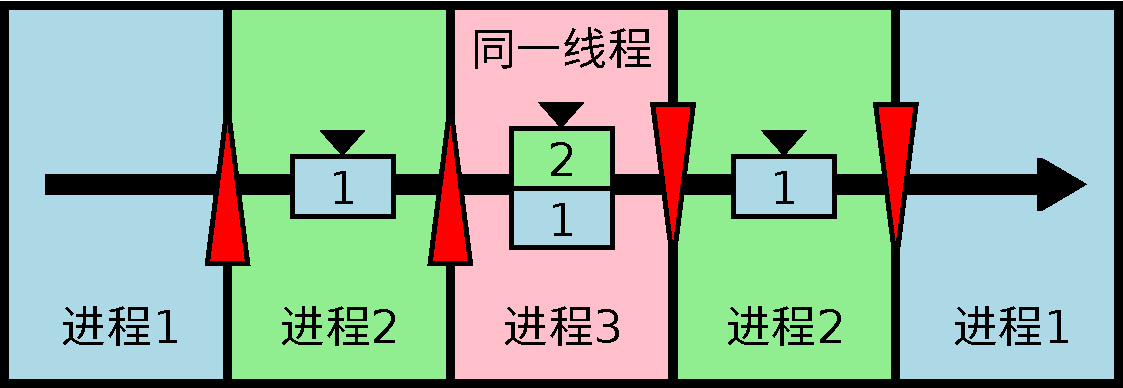
\includegraphics[width=0.72\textwidth]{Figure/image12.pdf}
    \caption{同步线程迁移示例}
    \label{fig:5-1-sync-thread-migration-example}
\end{figure}

同步迁移调用的设计参考了 Composite\hyperref[cite:5-1]{{[}1{]}}和 Mach 3\hyperref[cite:5-2]{{[}2{]}}。

\subsection{异步通信概述}\label{subsec:5-async-communication-overview}

操作系统中的异步（Asynchronous）通信机制是用来协调操作系统中的生产者-消费者（Producer-Consumer）问题的。通常而言这样的机制有邮箱（Mailbox）、消息队列（Message
Queue）等。异步通信机制的最大特点为其非阻塞性，也即一方发出后，另一方不接收，信息会先被缓存，然后发送者将直接返回。接收者在接收时，如果有信息，那么接收者返回；如果没有信息，那么接收者视系统调用的情况，可以直接返回，可以阻塞，也可以阻塞一段时间直到超时返回。

在 RME 中，异步通信模型被进一步简化为信号端点（Signal
Endpoint），其主要机制是使发送者可以向信号端点发送，使接收者可以从信号端点接收。发送总是不阻塞的，接收在有信号之时也是不阻塞的，接收在没有信号之时则可以阻塞也可以不阻塞。信号只携带数目信息\footnote{它只有一个计数器}，不携带任何其他信息。如果需要传递其他信息，那么需要在用户态通过共享内存（Shared
Memory）完成对这些信息的传递。一个异步通信的例子如下所示。其中优先级较低的线程1给优先级较高的线程2发送了一个异步信号（红色闪电标志），线程2在完成处理后又在端点上阻塞（红色长方形标志），使线程1继续执行。

\begin{figure}[htbp]
    \centering
    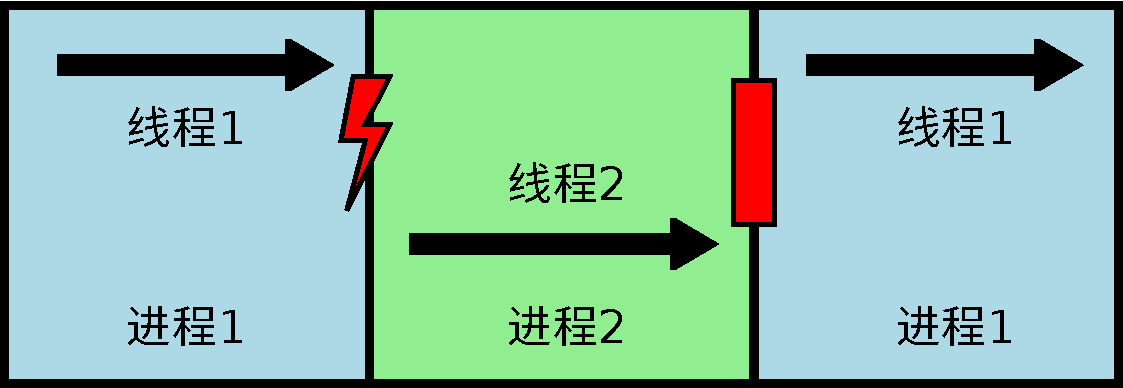
\includegraphics[width=0.72\textwidth]{Figure/image13.pdf}
    \caption{异步信号收发示例}
    \label{fig:5-2-async-signal-send-receive-example}
\end{figure}

\section{同步通信操作}\label{sec:5-sync-communication-operations}

要使用同步通信功能，那么需要先创建一个同步迁移调用。在创建同步迁移调用时，需要指明进程。在创建后，需要指定这个进程内部调用的入口和给该线程使用的栈。接下来，进行同步迁移调用，线程从一个线程内部过渡到另外一个进程之内执行。如果在这个同步迁移调用之中使用了其他的同步迁移调用，那么同步迁移调用将会进行嵌套（Nesting）。在同步迁移调用执行完毕之后，需要调用同步迁移调用返回功能，从这个迁移调用之中返回。和异步通信相比，同步通信操作具有即时性，保证在调用时一定会以最快速度得到响应，而且在进行调用时线程仅仅是跨到另外一个保护域中执行而不改变其其他属性。需要注意的是，同步迁移调用不会保存任何通用寄存器或者协处理器寄存器，也不会更改协处理器当前的状态；它只会更改那些改变程序执行流必要的寄存器，如堆栈指针和程序计数器等。通用寄存器的值和协处理器状态将会被直接带到线程迁移入口和出口。如果有需要保存的寄存器或者协处理器状态，那么需要用户态自行完成。此外，协处理器寄存器组也可以用来传递额外的参数或者接收额外的返回值。

同步迁移调用不会被绑定到CPU。如果有多个CPU上的线程试图同时激活一个同步迁移调用，那么只有一个CPU上的线程会成功，其他的线程都会返回错误码；如果在一个迁移调用被激活时试图再次激活它\footnote{不管是在同一个CPU上还是在不同的CPU上}，那么也会返回错误码。

如果同步迁移调用中发生了嵌套，那么返回时也需要逐级返回。如果线程在进行迁移调用的过程中被解除绑定，那么它仍然处于迁移调用状态，被绑定到新的CPU后会继续从那里执行；如果线程在进行迁移调用的过程中发生了一个错误，线程的行为是由设置迁移调用执行属性时传入的 Fault\_Ret\_Flag 参数决定的。如果该参数不为0，那么它并不会进入 RME\_THD\_EXCPEND 状态，而是会直接从这个迁移调用中返回到上一级，并且返回值是指示发生了错误的错误码。如果该参数为0，那么该线程会进入 RME\_THD\_EXCPEND 状态等待错误修复。

\section{异步通信操作}\label{sec:5-async-communication-operations}

要使用异步通信功能，那么需要先创建一个信号端点，然后使发送方向其发送信号，接收方从该端点接收即可。接收时，如果该端点没有信号，那么会阻塞；接收如果成功，那么返回值将会是顺利返回时的剩余信号数。

信号端点不会被绑定到CPU。如果有多个CPU上的线程同时试图阻塞在一个端点，那么只有一个会成功，其他的线程都会返回一个错误值。如果在一个线程已经阻塞在一个端点时，其他线程也试图阻塞\footnote{不管是在同一个CPU上还是在不同的CPU上}，那么其他线程的阻塞会失败。在实践中不推荐一个信号端点多接收者的使用方法，因为这往往需要相当复杂的协调。

需要注意的是，当一个线程已经阻塞在某个信号端点时，只有和被阻塞线程同一个CPU上的发送操作才能解除该线程的阻塞。其他CPU上的线程虽然也能向该端点发送，但是只能增加信号计数而无法解除阻塞。

RME 不允许初始（Init）线程接收任何信号。因为接收信号是潜在的阻塞操作，而 Init 线程一旦阻塞，RME 就无法保证能够在 CPU 空闲时找到一个线程来运行。如果既需要接收信号，又需要接收线程的时间片是无限的，那么可以新建一个线程，然后从 Init 向它进行无限传递，将其变成无限线程。

为了使应用程序的编写更加灵活，RME 允许四种不同的端点信号接收方法，分别如下：

\begin{xltabular}{\textwidth}{@{}>{\hsize=0.5583\hsize\raggedright\arraybackslash}X>{\hsize=1.4417\hsize\raggedright\arraybackslash}X@{}}
\caption{端点信号的四种接收方法}\label{tab:5-1-endpoint-signal-receive-methods}\\
\toprule
接收选项 & 意义\tabularnewline
\endfirsthead
\toprule
接收选项 & 意义\tabularnewline
\midrule
\endhead
\bottomrule
\endlastfoot
RME\_RCV\_BS &
以阻塞方式试图接收单个信号。有可能造成线程本身阻塞。\tabularnewline
RME\_RCV\_BM &
以阻塞方式试图接收多个信号。有可能造成线程本身阻塞，并且如果端点上有信号，会获取端点上全部的信号。\tabularnewline
RME\_RCV\_NS &
以非阻塞方式试图接收单个信号。该方法在端点上无信号时会立即返回。\tabularnewline
RME\_RCV\_NM &
以非阻塞方式试图接收多个信号。该方法在端点上无信号时会立即返回，并且如果端点上有信号，会获取端点上全部的信号。\tabularnewline
\end{xltabular}

\section{同步通信功能列表}\label{sec:5-sync-communication-function-list}

与同步迁移调用有关的内核功能如下：

\begin{xltabular}{\textwidth}{@{}>{\hsize=0.8854\hsize\raggedright\arraybackslash}X>{\hsize=0.6747\hsize\raggedright\arraybackslash}X>{\hsize=1.4400\hsize\raggedright\arraybackslash}X@{}}
\caption{同步通信相关内核功能}\label{tab:5-2-sync-communication-kernel-functions}\\
\toprule
调用号 & 类型 & 用途\tabularnewline
\endfirsthead
\toprule
调用号 & 类型 & 用途\tabularnewline
\midrule
\endhead
\bottomrule
\endlastfoot
RME\_SVC\_INV\_CRT & 系统调用 & 创建同步迁移调用\tabularnewline
RME\_SVC\_INV\_DEL & 系统调用 & 删除同步迁移调用\tabularnewline
RME\_SVC\_INV\_SET & 系统调用 &
设置同步迁移调用的执行属性\footnote{入口和栈}\tabularnewline
RME\_SVC\_INV\_ACT & 系统调用 &
激活\footnote{进行或调用}同步迁移调用\tabularnewline
RME\_SVC\_INV\_RET & 系统调用 & 从同步迁移调用返回\tabularnewline
\end{xltabular}

同步迁移调用权能的操作标志如下：

\begin{xltabular}{\textwidth}{@{}>{\hsize=0.9420\hsize\raggedright\arraybackslash}X>{\hsize=0.6957\hsize\raggedright\arraybackslash}X>{\hsize=1.3622\hsize\raggedright\arraybackslash}X@{}}
\caption{同步迁移调用操作标志}\label{tab:5-3-sync-invocation-operation-flags}\\
\toprule
标志 & 位 & 用途\tabularnewline
\endfirsthead
\toprule
标志 & 位 & 用途\tabularnewline
\midrule
\endhead
\bottomrule
\endlastfoot
RME\_INV\_FLAG\_SET & {[}0{]} &
允许设置该同步迁移调用的执行属性。\tabularnewline
RME\_INV\_FLAG\_ACT & {[}1{]} & 允许激活该同步迁移调用。\tabularnewline
\end{xltabular}

由于同步迁移调用返回操作是不需要同步迁移调用权能的，因此也没有该操作标志位\footnote{详见第~\ref{subsec:5-return-from-sync-invocation}~节}。

\subsection{创建同步迁移调用}\label{subsec:5-create-sync-invocation}

该操作会创建一个同步迁移调用，并将其权能放入某个已存在的权能表。新创建的同步迁移调用会引用创建时指定的进程，一旦在某进程内创建了一个同步迁移调用，那么这个进程在该同步迁移调用被删除前就不能被删除。创建同步迁移调用需要如下几个参数：

\begin{xltabular}{\textwidth}{@{}>{\hsize=0.6910\hsize\raggedright\arraybackslash}X>{\hsize=0.6910\hsize\raggedright\arraybackslash}X>{\hsize=0.6910\hsize\raggedright\arraybackslash}X>{\hsize=1.9271\hsize\raggedright\arraybackslash}X@{}}
\caption{创建同步迁移调用的所需参数}\label{tab:5-4-create-sync-invocation-parameters}\\
\toprule
参数名称 & 类型 & 域 & 描述\tabularnewline
\endfirsthead
\toprule
参数名称 & 类型 & 域 & 描述\tabularnewline
\midrule
\endhead
\bottomrule
\endlastfoot
Svc\_Num & ptr\_t & N & 必须为 RME\_SVC\_INV\_CRT。\tabularnewline
Cap\_Cpt & cid\_t & C &
一个对应于必须拥有 RME\_CPT\_FLAG\_CRT 属性的权能表权能的权能号，该权能号对应的权能指向要接受此新创建的同步迁移调用权能的权能表。该权能号可以是一级或者二级查找编码。\tabularnewline
Cap\_Kom & cid\_t & P1.D1 &
一个内核内存权能号，其标识的内核内存范围必须能够放下整个同步迁移调用对象，并且要拥有 RME\_KOM\_FLAG\_INV 属性。该权能号可以是一级或二级查找编码。\tabularnewline
Cap\_Inv & cid\_t & P1.D0 &
一个对应于接受该新创建的同步迁移调用权能的权能表的某位置的权能号。该权能号对应的权能必须是空白的。该权能号只能是一级查找编码。\tabularnewline
Cap\_Prc & cid\_t & P2 &
一个对应于必须拥有 RME\_PRC\_FLAG\_INV 属性的进程权能的权能号，该权能号对应的权能指向包含新创建的同步迁移调用的进程。该权能号可以是一级或者二级查找编码。\tabularnewline
Raddr & ptr\_t & P3 &
新创建的同步迁移调用要使用的内核起始相对虚拟地址。这个地址是相对于Cap\_Kom对应的内核权能的起始虚拟地址的。\tabularnewline
\end{xltabular}

该操作的返回值可能如下：

\begin{xltabular}{\textwidth}{@{}>{\hsize=0.8317\hsize\raggedright\arraybackslash}X>{\hsize=1.1683\hsize\raggedright\arraybackslash}X@{}}
\caption{同步迁移调用创建的可能返回值}\label{tab:5-5-create-sync-invocation-return-values}\\
\toprule
返回值 & 意义\tabularnewline
\endfirsthead
\toprule
返回值 & 意义\tabularnewline
\midrule
\endhead
\bottomrule
\endlastfoot
    0 & 操作成功。\tabularnewline
    RME\_ERR\_CPT\_RANGE & Cap\_Cpt 的一级/二级查找超出了范围。\tabularnewline
    RME\_ERR\_CPT\_RANGE & Cap\_Kom 的一级/二级查找超出了范围。\tabularnewline
    RME\_ERR\_CPT\_RANGE & Cap\_Prc 的一级/二级查找超出了范围。\tabularnewline
    RME\_ERR\_CPT\_RANGE & Cap\_Inv 的一级查找超出了范围。\tabularnewline
    RME\_ERR\_CPT\_FROZEN & Cap\_Cpt 的一级/二级查找的权能已经被冻结。\tabularnewline
    RME\_ERR\_CPT\_FROZEN & Cap\_Kom 的一级/二级查找的权能已经被冻结。\tabularnewline
    RME\_ERR\_CPT\_FROZEN & Cap\_Prc 的一级/二级查找权能已经被冻结。\tabularnewline
    RME\_ERR\_CPT\_FROZEN & Cap\_Inv 被冻结，或者其它核正在该处创建权能。\tabularnewline
    RME\_ERR\_CPT\_TYPE & Cap\_Cpt 不是权能表权能。\tabularnewline
    RME\_ERR\_CPT\_TYPE & Cap\_Kom 不是内核内存权能。\tabularnewline
    RME\_ERR\_CPT\_TYPE & Cap\_Prc 不是进程权能。\tabularnewline
    RME\_ERR\_CPT\_FLAG & Cap\_Cpt 无 RME\_CPT\_FLAG\_CRT 属性。\tabularnewline
    RME\_ERR\_CPT\_FLAG & Cap\_Kom 无 RME\_KOM\_FLAG\_INV 属性，或范围错误。\tabularnewline
    RME\_ERR\_CPT\_FLAG & Cap\_Prc 无 RME\_PRC\_FLAG\_INV 属性。\tabularnewline
    RME\_ERR\_CPT\_EXIST & Cap\_Inv 不是空白权能。\tabularnewline
    RME\_ERR\_CPT\_KOT & 分配内核内存失败。\tabularnewline
\end{xltabular}

\subsection{删除同步迁移调用}\label{subsec:5-delete-sync-invocation}

该操作会删除一个同步迁移调用。被删除的同步迁移调用必须不处于正被使用的状态。删除同步迁移调用需要如下几个参数：

\begin{xltabular}{\textwidth}{@{}>{\hsize=0.6910\hsize\raggedright\arraybackslash}X>{\hsize=0.6910\hsize\raggedright\arraybackslash}X>{\hsize=0.6910\hsize\raggedright\arraybackslash}X>{\hsize=1.9271\hsize\raggedright\arraybackslash}X@{}}
\caption{删除同步迁移调用的所需参数}\label{tab:5-6-delete-sync-invocation-parameters}\\
\toprule
参数名称 & 类型 & 域 & 描述\tabularnewline
\endfirsthead
\toprule
参数名称 & 类型 & 域 & 描述\tabularnewline
\midrule
\endhead
\bottomrule
\endlastfoot
Svc\_Num & ptr\_t & N & 必须为 RME\_SVC\_INV\_DEL。\tabularnewline
Cap\_Cpt & cid\_t & C &
一个对应于必须拥有 RME\_CPT\_FLAG\_DEL 属性的权能表权能的权能号，该权能号对应的权能指向含有正被删除的同步迁移调用权能的权能表。该权能号可以是一级或者二级查找编码。\tabularnewline
Cap\_Inv & cid\_t & P1 &
一个对应于将被删除的同步迁移调用权能的权能号。该权能号对应的必须是一个同步迁移调用权能。该权能号只能是一级查找编码。\tabularnewline
\end{xltabular}

该操作的返回值可能如下：

\begin{xltabular}{\textwidth}{@{}>{\hsize=0.7199\hsize\raggedright\arraybackslash}X>{\hsize=1.2801\hsize\raggedright\arraybackslash}X@{}}
\caption{删除同步迁移调用的可能返回值}\label{tab:5-7-delete-sync-invocation-return-values}\\
\toprule
返回值 & 意义\tabularnewline
\endfirsthead
\toprule
返回值 & 意义\tabularnewline
\midrule
\endhead
\bottomrule
\endlastfoot
    0 & 操作成功。\tabularnewline
    RME\_ERR\_CPT\_RANGE & Cap\_Cpt 的一级/二级查找超出了范围。\tabularnewline
    RME\_ERR\_CPT\_RANGE & Cap\_Inv 的一级查找超出了范围。\tabularnewline
    RME\_ERR\_CPT\_FROZEN & Cap\_Cpt 的一级/二级查找的权能已经被冻结。\tabularnewline
    RME\_ERR\_CPT\_FROZEN & Cap\_Inv 未被冻结。\tabularnewline
    RME\_ERR\_CPT\_TYPE & Cap\_Cpt 不是权能表权能。\tabularnewline
    RME\_ERR\_CPT\_TYPE & Cap\_Inv 不是同步迁移调用权能。\tabularnewline
    RME\_ERR\_CPT\_NULL & Cap\_Inv 为空白权能。\tabularnewline
    RME\_ERR\_CPT\_NULL & 两个核同时试图删除该同步迁移调用，此时未成功的核返回该值。\tabularnewline
    RME\_ERR\_CPT\_FLAG & Cap\_Cpt 无 RME\_CPT\_FLAG\_DEL 属性。\tabularnewline
    RME\_ERR\_CPT\_QUIE & Cap\_Inv 不安定。\tabularnewline
    RME\_ERR\_CPT\_REFCNT & Cap\_Inv 的引用计数不为 0，或者不为根权能。\tabularnewline
    RME\_ERR\_SIV\_ACT & 该同步迁移调用仍然处于被使用状态。\tabularnewline
\bottomrule
\end{xltabular}

\needspace{30\baselineskip}
\subsection{设置同步迁移调用执行属性}\label{subsec:5-set-sync-invocation-properties}

\needspace{20\baselineskip}
该操作会设置同步迁移调用的执行属性，也即其入口和栈。我们在设置时不关心该同步迁移调用是否已经在被使用。设置同步迁移调用的执行属性需要以下几个参数：

\begin{xltabular}{\textwidth}{@{}>{\hsize=0.7362\hsize\raggedright\arraybackslash}X>{\hsize=0.6815\hsize\raggedright\arraybackslash}X>{\hsize=0.6815\hsize\raggedright\arraybackslash}X>{\hsize=1.9007\hsize\raggedright\arraybackslash}X@{}}
\caption{设置同步迁移调用执行属性的所需参数}\label{tab:5-8-set-sync-invocation-properties-parameters}\\
\toprule
参数名称 & 类型 & 域 & 描述\tabularnewline
\endfirsthead
\toprule
参数名称 & 类型 & 域 & 描述\tabularnewline
\midrule
\endhead
Svc\_Num & ptr\_t & N & 必须为 RME\_SVC\_INV\_SET。\tabularnewline
Cap\_Inv & cid\_t & P1.D0 &
一个对应于必须拥有 RME\_INV\_FLAG\_SET 属性的同步迁移调用权能的权能号，该权能号对应的权能指向被设置执行属性的同步迁移调用。该权能号可以是一级或者二级查找编码。\tabularnewline
Entry & ptr\_t & P2 &
该线程迁移到用的入口。这个值是该同步迁移调用所在的进程内部的一个虚拟地址，同步迁移调用将从这里开始执行。\tabularnewline
Stack & ptr\_t & P3 &
该同步迁移调用的执行栈。这个值是该同步迁移调用所在的进程内部的一个虚拟地址，同步迁移调用将使用这个地址作为栈的起始。具体的栈是递增堆栈还是递减堆栈由用户态库决定。\tabularnewline
Is\_Exc\_Ret & ptr\_t & P1.D1 &
如果不为0，在迁移调用中一旦发生错误将会强制从迁移调用返回，不会允许错误修复。如果为0，则该线程将进入 RME\_THD\_EXCPEND 状态等待错误修复。\tabularnewline
\end{xltabular}

该操作的返回值可能如下：

\begin{xltabular}{\textwidth}{@{}>{\hsize=0.8188\hsize\raggedright\arraybackslash}X>{\hsize=1.1812\hsize\raggedright\arraybackslash}X@{}}
\caption{设置同步迁移调用执行属性的可能返回值}\label{tab:5-9-set-sync-invocation-properties-return-values}\\
\toprule
返回值 & 意义\tabularnewline
\endfirsthead
\toprule
返回值 & 意义\tabularnewline
\midrule
\endhead
\bottomrule
\endlastfoot
    0 & 操作成功。\tabularnewline
    RME\_ERR\_CPT\_RANGE & Cap\_Inv 的一级/二级查找超出了范围。\tabularnewline
    RME\_ERR\_CPT\_FROZEN & Cap\_Inv 的一级/二级查找的权能已经被冻结。\tabularnewline
    RME\_ERR\_CPT\_TYPE & Cap\_Inv 不是同步迁移调用权能，或者为空白权能。\tabularnewline
    RME\_ERR\_CPT\_FLAG & Cap\_Inv 无 RME\_INV\_FLAG\_SET 属性。\tabularnewline
\end{xltabular}

\subsection{激活同步迁移调用}\label{subsec:5-activate-sync-invocation}

该操作会进行一个同步迁移调用。该迁移调用必须没有被占用。进行同步迁移调用需要以下几个参数：

\begin{xltabular}{\textwidth}{@{}>{\hsize=0.6910\hsize\raggedright\arraybackslash}X>{\hsize=0.6910\hsize\raggedright\arraybackslash}X>{\hsize=0.6910\hsize\raggedright\arraybackslash}X>{\hsize=1.9271\hsize\raggedright\arraybackslash}X@{}}
\caption{激活同步迁移调用的所需参数}\label{tab:5-10-activate-sync-invocation-parameters}\\
\toprule
参数名称 & 类型 & 域 & 描述\tabularnewline
\endfirsthead
\toprule
参数名称 & 类型 & 域 & 描述\tabularnewline
\midrule
\endhead
\bottomrule
\endlastfoot
Svc\_Num & ptr\_t & N & 必须为 RME\_SVC\_INV\_ACT。\tabularnewline
Cap\_Inv & cid\_t & P1 &
一个对应于必须拥有 RME\_INV\_FLAG\_ACT 属性的同步迁移调用权能的权能号，该权能号对应的权能指向被要被激活的同步迁移调用。该权能号可以是一级或者二级查找编码。\tabularnewline
Param & ptr\_t & P2 & 要向该同步迁移调用传入的参数。\tabularnewline
\end{xltabular}

\needspace{20\baselineskip}
该操作的返回值可能如下：

\begin{xltabular}{\textwidth}{@{}>{\hsize=0.8788\hsize\raggedright\arraybackslash}X>{\hsize=1.1212\hsize\raggedright\arraybackslash}X@{}}
\caption{激活同步迁移调用的可能返回值}\label{tab:5-11-activate-sync-invocation-return-values}\\
\toprule
返回值 & 意义\tabularnewline
\endfirsthead
\toprule
返回值 & 意义\tabularnewline
\midrule
\endhead
\bottomrule
\endlastfoot
    0 & 操作成功。\tabularnewline
    RME\_ERR\_CPT\_RANGE & Cap\_Inv 的一级/二级查找超出了范围。\tabularnewline
    RME\_ERR\_CPT\_FROZEN & Cap\_Inv 的一级/二级查找的权能已经被冻结。\tabularnewline
    RME\_ERR\_CPT\_TYPE & Cap\_Inv 不是同步迁移调用权能，或者为空白权能。\tabularnewline
    RME\_ERR\_CPT\_FLAG & Cap\_Inv 无 RME\_INV\_FLAG\_ACT 属性。\tabularnewline
    RME\_ERR\_SIV\_ACT & 只有当 RME\_INV\_DEPTH\_MAX\footnote{见 7.3.2} 不为 0 时可能发生：若激活该同步迁移调用，则当前线程的总调用深度会超过该上限。\tabularnewline
    RME\_ERR\_SIV\_ACT & Cap\_Inv 已经在激活状态\footnote{其他线程正在进行调用}。\tabularnewline
    RME\_ERR\_SIV\_ACT & 两个 CPU 试图同时进行这个调用，失败的 CPU 返回该值。\tabularnewline
\end{xltabular}

\subsection{从同步迁移调用返回}\label{subsec:5-return-from-sync-invocation}

该操作从一个同步迁移调用返回。这是一个特殊操作，它不需要除了调用号和线程迁移返回值之外的其他参数。如果有多个同步迁移调用嵌套，该函数返回到上一级同步迁移调用中。如果试图在没有同步迁移调用的情况下调用该函数，则会返回一个错误码，标志着返回未成功。从同步迁移调用返回需要如下参数：

\begin{xltabular}{\textwidth}{@{}>{\hsize=1.0000\hsize\raggedright\arraybackslash}X>{\hsize=1.0000\hsize\raggedright\arraybackslash}X>{\hsize=1.0000\hsize\raggedright\arraybackslash}X>{\hsize=1.0000\hsize\raggedright\arraybackslash}X@{}}
\caption{从同步迁移调用返回的所需参数}\label{tab:5-12-return-from-sync-invocation-parameters}\\
\toprule
参数名称 & 类型 & 域 & 描述\tabularnewline
\endfirsthead
\toprule
参数名称 & 类型 & 域 & 描述\tabularnewline
\midrule
\endhead
\bottomrule
\endlastfoot
Svc\_Num & ptr\_t & N & 必须为 RME\_SVC\_INV\_RET。\tabularnewline
\end{xltabular}

该操作的返回值可能如下：

\begin{xltabular}{\textwidth}{@{}>{\hsize=0.7151\hsize\raggedright\arraybackslash}X>{\hsize=1.2849\hsize\raggedright\arraybackslash}X@{}}
\caption{从同步迁移调用返回的可能返回值}\label{tab:5-13-return-from-sync-invocation-return-values}\\
\toprule
返回值 & 意义\tabularnewline
\endfirsthead
\toprule
返回值 & 意义\tabularnewline
\midrule
\endhead
\bottomrule
\endlastfoot
    0 & 操作成功。该迁移调用立即返回，该返回值不会被调用者接收。\tabularnewline
    RME\_ERR\_SIV\_EMPTY & 试图在没有同步迁移调用的情况下调用该函数。\tabularnewline
\end{xltabular}

\section{异步通信功能列表}\label{sec:5-async-communication-function-list}

与信号端点有关的内核功能如下：

\begin{xltabular}{\textwidth}{@{}>{\hsize=1.0112\hsize\raggedright\arraybackslash}X>{\hsize=0.7705\hsize\raggedright\arraybackslash}X>{\hsize=1.2183\hsize\raggedright\arraybackslash}X@{}}
\caption{异步通信相关内核功能}\label{tab:5-14-async-communication-kernel-functions}\\
\toprule
调用号 & 类型 & 用途\tabularnewline
\endfirsthead
\toprule
调用号 & 类型 & 用途\tabularnewline
\midrule
\endhead
\bottomrule
\endlastfoot
RME\_SVC\_SIG\_CRT & 系统调用 & 创建异步信号端点\tabularnewline
RME\_SVC\_SIG\_DEL & 系统调用 & 删除异步信号端点\tabularnewline
RME\_SVC\_SIG\_SND & 系统调用 & 向异步信号端点发送信号\tabularnewline
RME\_SVC\_SIG\_RCV & 系统调用 & 从异步信号端点接收信号\tabularnewline
\end{xltabular}

信号端点权能的操作标志如下：

\begin{xltabular}{\textwidth}{@{}>{\hsize=0.9507\hsize\raggedright\arraybackslash}X>{\hsize=0.6459\hsize\raggedright\arraybackslash}X>{\hsize=1.4035\hsize\raggedright\arraybackslash}X@{}}
\caption{信号端点操作标志}\label{tab:5-15-signal-endpoint-operation-flags}\\
\toprule
标志 & 位 & 用途\tabularnewline
\endfirsthead
\toprule
标志 & 位 & 用途\tabularnewline
\midrule
\endhead
\bottomrule
\endlastfoot
RME\_SIG\_FLAG\_SND & {[}0{]} & 允许向该信号端点发送。\tabularnewline
RME\_SIG\_FLAG\_RCV\_BS & {[}1{]} &
允许从该信号端点以阻塞方式接收单个信号。\tabularnewline
RME\_SIG\_FLAG\_RCV\_BM & {[}2{]} &
允许从该信号端点以阻塞方式接收多个信号。\tabularnewline
RME\_SIG\_FLAG\_RCV\_NS & {[}3{]} &
允许从该信号端点以非阻塞方式接收单个信号。\tabularnewline
RME\_SIG\_FLAG\_RCV\_NM & {[}4{]} &
允许从该信号端点以非阻塞方式接收多个信号。\tabularnewline
RME\_SIG\_FLAG\_SCHED & {[}5{]} &
允许该端点被线程绑定用于调度器信号端点。\tabularnewline
\end{xltabular}

关于位{[}5{]}的描述，请参见\ref{subsec:4-receive-thread-scheduler-event}
。

\subsection{创建异步信号端点}\label{subsec:5-create-async-signal-endpoint}

\needspace{20\baselineskip}
该操作会创建一个信号端点，并将其权能放入某个已存在的权能表。创建信号端点需要如下几个参数：

\begin{xltabular}{\textwidth}{@{}>{\hsize=0.6910\hsize\raggedright\arraybackslash}X>{\hsize=0.6910\hsize\raggedright\arraybackslash}X>{\hsize=0.6910\hsize\raggedright\arraybackslash}X>{\hsize=1.9271\hsize\raggedright\arraybackslash}X@{}}
\caption{创建信号端点的所需参数}\label{tab:5-16-create-signal-endpoint-parameters}\\
\toprule
参数名称 & 类型 & 域 & 描述\tabularnewline
\endfirsthead
\toprule
参数名称 & 类型 & 域 & 描述\tabularnewline
\midrule
\endhead
\bottomrule
\endlastfoot
Svc\_Num & ptr\_t & N & 必须为 RME\_SVC\_SIG\_CRT。\tabularnewline
Cap\_Cpt & cid\_t & C &
一个对应于必须拥有 RME\_CPT\_FLAG\_CRT 属性的权能表权能的权能号，该权能号对应的权能指向要接受此新创建的信号端点权能的权能表。该权能号可以是一级或者二级查找编码。\tabularnewline
Cap\_Sig & cid\_t & P0 &
一个对应于接受该新创建的信号端点权能的权能表的某位置的权能号。该权能号对应的权能必须是空白的。该权能号只能是一级查找编码。\tabularnewline
\end{xltabular}

该操作的返回值可能如下：

\begin{xltabular}{\textwidth}{@{}>{\hsize=0.8317\hsize\raggedright\arraybackslash}X>{\hsize=1.1683\hsize\raggedright\arraybackslash}X@{}}
\caption{创建异步信号端点的可能返回值}\label{tab:5-17-create-signal-endpoint-return-values}\\
\toprule
返回值 & 意义\tabularnewline
\endfirsthead
\toprule
返回值 & 意义\tabularnewline
\midrule
\endhead
\bottomrule
\endlastfoot
    0 & 操作成功。\tabularnewline
    RME\_ERR\_CPT\_RANGE & Cap\_Cpt 的一级/二级查找超出了范围。\tabularnewline
    RME\_ERR\_CPT\_RANGE & Cap\_Sig 的一级查找超出了范围。\tabularnewline
    RME\_ERR\_CPT\_FROZEN & Cap\_Cpt 的一级/二级查找的权能已经被冻结。\tabularnewline
    RME\_ERR\_CPT\_FROZEN & Cap\_Sig 被冻结，或者其它核正在该处创建权能。\tabularnewline
    RME\_ERR\_CPT\_TYPE & Cap\_Cpt 不是权能表权能。\tabularnewline
    RME\_ERR\_CPT\_FLAG & Cap\_Cpt 无 RME\_CPT\_FLAG\_CRT 属性。\tabularnewline
    RME\_ERR\_CPT\_EXIST & Cap\_Sig 不是空白权能。\tabularnewline
\end{xltabular}

\subsection{删除异步信号端点}\label{subsec:5-delete-async-signal-endpoint}

该操作会删除一个信号端点。被删除的信号端点必须不处于正被使用\footnote{有线程阻塞在其上}的状态。删除信号端点需要如下几个参数：

\begin{xltabular}{\textwidth}{@{}>{\hsize=0.6910\hsize\raggedright\arraybackslash}X>{\hsize=0.6910\hsize\raggedright\arraybackslash}X>{\hsize=0.6910\hsize\raggedright\arraybackslash}X>{\hsize=1.9271\hsize\raggedright\arraybackslash}X@{}}
\caption{删除异步信号端点的所需参数}\label{tab:5-18-delete-signal-endpoint-parameters}\\
\toprule
参数名称 & 类型 & 域 & 描述\tabularnewline
\endfirsthead
\toprule
参数名称 & 类型 & 域 & 描述\tabularnewline
\midrule
\endhead
\bottomrule
\endlastfoot
Svc\_Num & ptr\_t & N & 必须为 RME\_SVC\_SIG\_DEL。\tabularnewline
Cap\_Cpt & cid\_t & C &
一个对应于必须拥有 RME\_CPT\_FLAG\_DEL 属性的权能表权能的权能号，该权能号对应的权能指向含有正被删除的信号端点权能的权能表。该权能号可以是一级或者二级查找编码。\tabularnewline
Cap\_Sig & cid\_t & P1 &
一个对应于将被删除的信号端点权能的权能号。该权能号对应的必须是一个信号端点权能。该权能号只能是一级查找编码。\tabularnewline
\end{xltabular}

该操作的返回值可能如下：

\begin{xltabular}{\textwidth}{@{}>{\hsize=0.7603\hsize\raggedright\arraybackslash}X>{\hsize=1.2397\hsize\raggedright\arraybackslash}X@{}}
\caption{删除异步信号端点的可能返回值}\label{tab:5-19-delete-signal-endpoint-return-values}\\
\toprule
返回值 & 意义\tabularnewline
\endfirsthead
\toprule
返回值 & 意义\tabularnewline
\midrule
\endhead
\bottomrule
\endlastfoot
    0 & 操作成功。\tabularnewline
    RME\_ERR\_CPT\_RANGE & Cap\_Cpt 的一级/二级查找超出了范围。\tabularnewline
    RME\_ERR\_CPT\_RANGE & Cap\_Sig 的一级查找超出了范围。\tabularnewline
    RME\_ERR\_CPT\_FROZEN & Cap\_Cpt 的一级/二级查找的权能已经被冻结。\tabularnewline
    RME\_ERR\_CPT\_FROZEN & Cap\_Sig 未被冻结。\tabularnewline
    RME\_ERR\_CPT\_TYPE & Cap\_Cpt 不是权能表权能。\tabularnewline
    RME\_ERR\_CPT\_TYPE & Cap\_Sig 不是信号端点权能。\tabularnewline
    RME\_ERR\_CPT\_NULL & Cap\_Sig 为空白权能。\tabularnewline
    RME\_ERR\_CPT\_NULL & 两个核同时试图删除该信号端点，此时未成功的核返回该值。\tabularnewline
    RME\_ERR\_CPT\_FLAG & Cap\_Cpt 无 RME\_CPT\_FLAG\_DEL 属性。\tabularnewline
    RME\_ERR\_CPT\_QUIE & Cap\_Sig 不安定。\tabularnewline
    RME\_ERR\_CPT\_REFCNT & Cap\_Sig 的引用计数不为 0，或者不为根权能。\tabularnewline
    RME\_ERR\_SIV\_ACT & 该信号端点仍然处于被使用状态。\tabularnewline
    RME\_ERR\_SIV\_CONFLICT & 该信号端点是一个内核端点，不能被删除。具体描述见下章。\tabularnewline
\end{xltabular}

\needspace{30\baselineskip}
\subsection{向异步信号端点发送信号}\label{subsec:5-send-signal-to-signal-endpoint}
\nopagebreak[4]

该操作会向一个信号端点发送信号。当有线程在该端点上阻塞时，只有与该线程相同CPU上的发送才能唤醒该线程。其他CPU也可以向该端点发送，但仅能增加计数值而不能唤醒该线程。向一个信号端点发送信号需要如下几个参数：

\begin{xltabular}{\textwidth}{@{}>{\hsize=0.6910\hsize\raggedright\arraybackslash}X>{\hsize=0.6910\hsize\raggedright\arraybackslash}X>{\hsize=0.6910\hsize\raggedright\arraybackslash}X>{\hsize=1.9271\hsize\raggedright\arraybackslash}X@{}}
\caption{向异步信号端点发送信号的所需参数}\label{tab:5-20-send-signal-parameters}\\
\toprule
参数名称 & 类型 & 域 & 描述\tabularnewline
\endfirsthead
\toprule
参数名称 & 类型 & 域 & 描述\tabularnewline
\midrule
\endhead
\bottomrule
\endlastfoot
Svc\_Num & ptr\_t & N & 必须为 RME\_SVC\_SIG\_SND。\tabularnewline
Cap\_Sig & cid\_t & P1 &
一个对应于必须拥有 RME\_SIG\_FLAG\_SND 属性的信号端点权能的权能号，该权能号对应的权能指向要对其发送信号的端点。该权能号可以是一级或者二级查找编码。\tabularnewline
Number & ptr\_t & P2 &
向信号端点发送的计数数量。一次能发送的数量上限在32位系统中为2\textsuperscript{16}，64位系统中则为2\textsuperscript{32}，依此类推。除了常规用途之外，当确信所有发送者和接收者均位于同一CPU核心、接收者优先级总是比任一发送者高时，接收者解除阻塞时会立即抢占发送者，该数字可以用来携带关于发送者身份的信息，以省去不必要的共享内存。\tabularnewline
\end{xltabular}

该操作的返回值可能如下：

\begin{xltabular}{\textwidth}{@{}>{\hsize=0.6791\hsize\raggedright\arraybackslash}X>{\hsize=1.3209\hsize\raggedright\arraybackslash}X@{}}
\caption{向异步信号端点发送信号的可能返回值}\label{tab:5-21-send-signal-return-values}\\
\toprule
返回值 & 意义\tabularnewline
\endfirsthead
\toprule
返回值 & 意义\tabularnewline
\midrule
\endhead
\bottomrule
\endlastfoot
    0 & 操作成功。\tabularnewline
    RME\_ERR\_CPT\_RANGE & Cap\_Sig 的一级/二级查找超出了范围。\tabularnewline
    RME\_ERR\_CPT\_FROZEN & Cap\_Sig 的一级/二级查找的权能已经被冻结。\tabularnewline
    RME\_ERR\_CPT\_TYPE & Cap\_Sig 不是信号端点权能，或为空白权能。\tabularnewline
    RME\_ERR\_CPT\_FLAG & Cap\_Sig 无 RME\_SIG\_FLAG\_SND 属性。\tabularnewline
    RME\_ERR\_SIV\_FULL & 发送的数量超过了一次能发送的数量上限。\tabularnewline
    RME\_ERR\_SIV\_FULL & 该信号端点的信号计数已满，不能再向其继续发送。这是很罕见的，因为在32位系统中信号计数的上限为2\textsuperscript{32-2}，64位系统中则为2\textsuperscript{64-2}，依此类推。\tabularnewline
\end{xltabular}

\subsection{从异步信号端点接收信号}\label{subsec:5-receive-signal-from-signal-endpoint}

该操作会从一个信号端点接收信号。如果该信号端点上没有信号，那么会阻塞该线程直到信号到来为止。从一个信号端点接收信号需要如下几个参数：

\begin{xltabular}{\textwidth}{@{}>{\hsize=0.6910\hsize\raggedright\arraybackslash}X>{\hsize=0.6910\hsize\raggedright\arraybackslash}X>{\hsize=0.6910\hsize\raggedright\arraybackslash}X>{\hsize=1.9271\hsize\raggedright\arraybackslash}X@{}}
\caption{从异步信号端点接收信号的所需参数}\label{tab:5-22-receive-signal-parameters}\\
\toprule
参数名称 & 类型 & 域 & 描述\tabularnewline
\endfirsthead
\toprule
参数名称 & 类型 & 域 & 描述\tabularnewline
\midrule
\endhead
\bottomrule
\endlastfoot
Svc\_Num & ptr\_t & N & 必须为 RME\_SVC\_SIG\_RCV。\tabularnewline
Cap\_Sig & cid\_t & P1 &
一个对应于必须拥有 RME\_SIG\_FLAG\_RCV 属性的信号端点权能的权能号，该权能号对应的权能指向要从其接收信号的端点。该权能号可以是一级或者二级查找编码。\tabularnewline
Option\strut
 & ptr\_t\strut
 & P2\strut
 & 接收方式选项。可以有以下四种方法：

RME\_RCV\_BS：阻塞并试图接收单个信号（Blocking Single）。

RME\_RCV\_BM：阻塞并试图接收多个信号（Blocking Multi）。

RME\_RCV\_NS：不阻塞并试图接收单个信号（Non-blocking Single）。

RME\_RCV\_NM：不阻塞并试图接收多个信号（Non-blocking Multi）。\strut
\tabularnewline
\end{xltabular}

该操作的返回值可能如下：

\begin{xltabular}{\textwidth}{@{}>{\hsize=0.7023\hsize\raggedright\arraybackslash}X>{\hsize=1.2977\hsize\raggedright\arraybackslash}X@{}}
\caption{从异步信号端点接收信号的可能返回值}\label{tab:5-23-receive-signal-return-values}\\
\toprule
返回值 & 意义\tabularnewline
\endfirsthead
\toprule
返回值 & 意义\tabularnewline
\midrule
\endhead
\bottomrule
\endlastfoot
    非负值 & 操作成功。该值为本次接收接收到的信号数量。\tabularnewline
    RME\_ERR\_CPT\_RANGE & Cap\_Sig 的一级/二级查找超出了范围。\tabularnewline
    RME\_ERR\_CPT\_FROZEN & Cap\_Sig 的一级/二级查找的权能已经被冻结。\tabularnewline
    RME\_ERR\_CPT\_TYPE & Cap\_Sig 不是信号端点权能，或为空白权能。\tabularnewline
    RME\_ERR\_CPT\_FLAG & Cap\_Sig 无对应的接收选项需要的属性。\tabularnewline
    RME\_ERR\_CPT\_FLAG & RME\_RCV\_BS 需要 RME\_SIG\_FLAG\_RCV\_BS 属性。\tabularnewline
    RME\_ERR\_CPT\_FLAG & RME\_RCV\_BM 需要 RME\_SIG\_FLAG\_RCV\_BM 属性。\tabularnewline
    RME\_ERR\_CPT\_FLAG & RME\_RCV\_NS 需要 RME\_SIG\_FLAG\_RCV\_NS 属性。\tabularnewline
    RME\_ERR\_CPT\_FLAG & RME\_RCV\_NM 需要 RME\_SIG\_FLAG\_RCV\_NM 属性。\tabularnewline
    RME\_ERR\_SIV\_BOOT & 试图让 Init 线程从端点以阻塞方式接收信号。\tabularnewline
    RME\_ERR\_SIV\_ACT & 已经有一个线程阻塞在该端点，无法接收信号。\tabularnewline
    RME\_ERR\_SIV\_ACT & 提供的接收选项不正确。\tabularnewline
    RME\_ERR\_SIV\_CONFLICT & 两个核试图同时在一个端点上进行接收，发生了冲突，需要重试。\tabularnewline
\end{xltabular}

需要注意的是，如果选择非阻塞方式，那么当该端点上无信号时，函数会直接返回0，代表此次接收没有收到任何东西。此外，如果接收选项是阻塞并试图接收多个信号，而且此次接收的确产生了阻塞，那么在阻塞解除时不论已经存在多少信号，接收的信号数目总是等于解除阻塞的那次发送。

\section{本章参考文献}\label{sec:5-references}

\protect\phantomsection\label{cite:5-1}
{[}1{]}
Q. Wang, Y. Ren, M. Scaperoth, and G. Parmer, "Speck: A kernel for
scalable predictability," in Real-Time and Embedded Technology and
Applications Symposium (RTAS), 2015 IEEE, 2015, pp. 121-132.

\protect\phantomsection\label{cite:5-2}
{[}2{]} B. Ford and J. Lepreau, "Evolving mach 3.0 to a migrating thread
model," presented at the Proceedings of the USENIX Winter 1994 Technical
Conference on USENIX Winter 1994 Technical Conference, San Francisco,
California, 1994.

